\documentclass[11pt]{article}

\usepackage[margin=1in]{geometry}
\usepackage{times}
\usepackage{amsmath,amssymb}
\usepackage{graphicx}
\usepackage{booktabs}
\usepackage{multirow}
\usepackage[hidelinks]{hyperref}
\usepackage[T1]{fontenc}
\usepackage{caption}
\usepackage{enumitem}
\usepackage{fancyhdr}
\usepackage{titlesec}
\usepackage{url}
\Urlmuskip=0mu plus 1mu
\usepackage{subcaption}
\clubpenalty=10000
\widowpenalty=10000
\raggedbottom

\titleformat{\section}{\normalfont\Large\bfseries}{\thesection}{1em}{}
\titleformat{\subsection}{\normalfont\large\bfseries}{\thesubsection}{1em}{}
\titleformat{\subsubsection}{\normalfont\bfseries}{\thesubsubsection}{1em}{}

\pagestyle{fancy}
\fancyhf{}
\fancyhead[C]{\small\itshape Certified Optimality and Structural Bottleneck Analysis for Indoor Evacuation QUBO Routing}
\fancyfoot[C]{\thepage}
\renewcommand{\headrulewidth}{0.4pt}

\title{\textbf{Certified Optimality Gaps and Structural Bottleneck Analysis \\
for Capacity-Aware Indoor Evacuation Route Assignment \\
Using QUBO Optimization and Quantum Annealing}}

\author{
Arielle Jenna Fishman \\
\small Florida Atlantic University \\
\small Machine Perception and Cognitive Robotics Laboratory
\and
Natalia Romero, Ph.D. \\
\small Florida Atlantic University \\
\small Machine Perception and Cognitive Robotics Laboratory
}
\date{August 2026}

\begin{document}
\maketitle

\begin{abstract}
This paper formulates static indoor evacuation-route assignment as a capacity-aware Quadratic Unconstrained Binary Optimization (QUBO) problem, solves it with classical simulated annealing, D-Wave Leap Hybrid, and direct quantum annealing across five real building floorplans (16 to 264 logical variables), and then goes further than prior work of this kind in three ways. First, we derive an exact, certified global optimum for \emph{every} floorplan -- not only the smallest -- by observing that the same objective, freed from its penalty-method exactly-one constraint, is a convex integer quadratic program, solvable directly and exactly with a general-purpose MIQP solver in under two seconds per instance. This reveals that Neal and D-Wave Hybrid, previously reported as producing good solutions, are in fact 94--124\% above the true optimum on two of the five floorplans, a gap invisible without a certified baseline. Second, we investigate why: a controlled compute-budget experiment (up to 100$\times$ the original sweep count) fails to close the gap, ruling out under-sampling, while a structural/geometric analysis and an 18-floorplan synthetic corpus with independently controlled corridor topology (linear, branching, and looped) identify \emph{corridor diameter} -- not bridge/bottleneck-edge count, our initial hypothesis -- as a predictor comparably strong to raw problem size ($r\approx0.83$) that nonetheless captures independent information, adding up to 13 additional percentage points of explained variance beyond variable count alone in a joint regression. This finding replicates under both classical and hybrid quantum solvers with proper significance testing (Mann-Whitney $U$, Bonferroni-corrected across 23 floorplans). Third, we report formal significance tests throughout, correcting the descriptive-statistics-only limitation of the original study. The result is a fully reproducible evacuation-QUBO workflow with, for the first time in this line of work, certified rather than merely observed solution quality, and an empirically grounded, statistically confirmed account of what makes a floorplan hard for current annealing-based solvers.
\end{abstract}

\noindent\textbf{Keywords} --- evacuation routing, QUBO, quantum annealing, capacity-aware optimization, minor embedding, certified optimality, mixed-integer programming, D-Wave, simulated annealing

\section{Introduction}

Emergency evacuation planning requires people to move from occupied spaces to safe exits along legal and understandable routes. Practical evacuation guidance emphasizes clearly identified exits, unobstructed routes, and floorplans that show how occupants can leave a building without entering hazardous or inaccessible areas \cite{osha}. From an optimization perspective, however, assigning every room to its individually nearest exit can concentrate many occupants on the same doorway or corridor. A short route for each individual group is therefore not necessarily the best coordinated assignment for the building as a whole.

Building evacuation has long been represented as a network problem with nodes, arcs, capacities, and bottlenecks \cite{chalmet}. Classical facility-to-exit assignment work also shows that coordinated assignments can outperform simple nearest-exit rules \cite{kang}. Modern indoor guidance methods incorporate corridor capacity, congestion, risk, and changing conditions \cite{desmet,zhang,ye}. These approaches motivate a system-level objective that balances route efficiency against shared infrastructure rather than minimizing geometric distance alone.

The Machine Perception and Cognitive Robotics Laboratory fellowship notebooks develop a progression from identifying binary decisions, objectives, and constraints to building Binary Quadratic Models (BQMs), sampling them with classical simulated annealing, and executing them on D-Wave Hybrid and direct quantum hardware. The original capstone project applied that progression to a larger original problem: representing five building layouts as validated wall-aware graphs, precomputing one legal route for each room-exit pair, and formulating the global assignment as a QUBO whose pairwise interactions penalize occupancy concentration on shared low-capacity edges.

That original study asked how effectively classical simulated annealing, a cloud Hybrid solver, and direct quantum annealing solve this QUBO as floorplan size and logical connectivity increase, and reported energy, physical route metrics, feasibility, runtime, and direct-QPU embedding behavior across 390 repeated solver runs. It found Hybrid consistently outperforming Neal, exact global optimality confirmed by exhaustive enumeration for the smallest 8-room floorplan, and two floorplans (FP02, FP03) whose density prevented direct embedding on the QPU altogether -- but it explicitly acknowledged, as a limitation, that results for the four larger floorplans were \emph{lowest observed energies, not certified optima}, and that no exact MIQP/MILP baseline or formal significance test was included.

This paper closes both of those gaps, and in doing so substantially revises the picture the original results supported. We show that the same congestion objective, once separated from the penalty method used to make it QUBO-solvable, is a convex integer quadratic program that a general-purpose solver certifies to global optimality in under two seconds for every floorplan tested, including the two that could not be embedded on the QPU at all. Measured against these certified optima rather than each other, Neal and Hybrid are far from the optimum on exactly the two floorplans the original study already flagged as structurally unusual -- landing 94--124\% above true optimal, roughly double, rather than the small margins their mutual comparison suggested. We then investigate why, first ruling out insufficient compute budget directly (a 100$\times$ sweep-count increase does not close the gap), then building a geometric/topological analysis of the floorplans' navigation graphs, and finally constructing an 18-floorplan synthetic corpus with independently controlled corridor topology to test candidate structural explanations under conditions the five real floorplans cannot provide. The result corrects our own initial hypothesis (bridge/bottleneck-edge count) in favor of a cleaner, better-supported one (corridor diameter), replicated with proper significance testing under both solvers evaluated.

The contributions are:
\begin{itemize}[leftmargin=*]
\item A reproducible wall-aware floorplan-to-graph workflow for five indoor building layouts (retained from the original study).
\item A room-group QUBO combining normalized route distance with occupancy-weighted, capacity-normalized shared-edge congestion (retained from the original study).
\item A controlled comparison of Neal simulated annealing, D-Wave Leap Hybrid, and direct-QPU execution using repeated independent runs (retained from the original study).
\item \textbf{New:} an exact convex-MIQP reformulation certifying the global optimum for all five floorplans -- not only the smallest -- solved in under two seconds each, exposing optimality gaps of 94--124\% on two floorplans that a solver-vs-solver comparison alone cannot reveal.
\item \textbf{New:} formal significance testing (Mann-Whitney $U$, Bonferroni-corrected) replacing the descriptive-statistics-only comparison of the original study.
\item \textbf{New:} a root-cause investigation combining a direct compute-budget ablation (ruling out under-sampling) with a three-part structural bottleneck taxonomy (capacity, traffic-concentration, and topological) applied to the floorplans' raw navigation graphs.
\item \textbf{New:} an 18-floorplan synthetic corpus with independently controlled corridor topology, used to test the structural hypothesis under conditions the original five floorplans cannot provide, statistically confirming corridor diameter (not bridge count, our initial hypothesis) as the dominant structural predictor of optimality gap, replicated under both Neal and Hybrid.
\end{itemize}

\section{Related Work}

\subsection{Building evacuation networks and exit assignment}
Chalmet, Francis, and Saunders developed foundational network models for building evacuation in which occupants move through capacity-limited arcs toward exits \cite{chalmet}. Kang, Jeong, and Kwun later formulated a closely related facility-final exit assignment problem, where rooms or other building subspaces are assigned to known routes leading to exterior exits \cite{kang}. Their integer model keeps occupants associated with a facility together, while a linear variant allows splitting. This structure is an important classical predecessor to the present room-group formulation.

The NIST review by Kuligowski, Peacock, and Hoskins places route optimization within a broader evacuation-modeling landscape that may include pre-movement delay, individual behavior, smoke and fire effects, exit blockage, group movement, and validation against experiments \cite{kuligowski}. The present work addresses only the route-assignment layer.

\subsection{Capacity-, congestion-, and risk-aware routing}
Desmet and Gelenbe proposed capacity-based evacuation guidance with dynamic exit signs \cite{desmet}. Zhang et al. developed congestion-aware indoor evacuation routing using augmented-reality devices \cite{zhang}. Pedestrian bottleneck research shows exit throughput depends on geometry, crowd formation, and incoming flow rather than a single universal capacity value \cite{ye}. Accordingly, the capacities used here are relative prototype values for optimization experiments, not empirically calibrated pedestrian flow rates.

\subsection{Classical path generation and direct shortest-path QUBOs}
Dijkstra's algorithm provides shortest paths on graphs with nonnegative edge weights \cite{dijkstra}, while A* uses a heuristic to guide search \cite{astar}. Krauss and McCollum encode the shortest-path problem itself into a QUBO \cite{krauss}. The present two-stage design instead reduces the logical decision to selecting among already-valid routes, reserving quadratic interactions for system-level congestion and assignment.

\subsection{QUBO, traffic assignment, and quantum evacuation}
Lucas provides general Ising and QUBO constructions for many discrete optimization problems \cite{lucas}. Neukart et al. applied quantum annealing to traffic-flow optimization by selecting candidate routes while penalizing shared road segments \cite{neukart}. Shikanai et al. provide the closest recent comparison: a large-scale vehicle-evacuation formulation choosing among pre-generated candidate routes while balancing travel distance and route overlap under a one-route-per-vehicle constraint \cite{shikanai}. The present project adapts that general route-selection structure to indoor building graphs and room-level occupant groups, weighting shared edges by room occupancy and normalizing load by modeled edge capacity.

\subsection{Exact and certified baselines for QUBO-formulated problems}
A recurring, explicitly acknowledged limitation across this literature -- including the original version of the present study -- is the absence of an exact classical baseline: results are reported as best-observed energy across repeated solver runs, without a certificate that no better solution exists. Where the underlying combinatorial structure is convex once separated from its penalty-method encoding, as we show is the case here, general-purpose mixed-integer quadratic programming solvers such as Google OR-Tools CP-SAT \cite{ortools} can supply that certificate directly, without embedding, chaining, or penalty tuning. We are not aware of prior work in the quantum-evacuation-routing literature that reports certified rather than observed optima across a full floorplan benchmark.

\subsection{Research gap and positioning}
Existing research has established network-flow evacuation models, facility-to-exit assignment, congestion-aware indoor routing, direct shortest-path QUBOs, quantum traffic assignment, and quantum evacuation-route selection, but not combined with certified optimality baselines, formal significance testing, and a controlled structural analysis of \emph{why} certain floorplan topologies resist QUBO-based optimization. This paper addresses that intersection. It does not claim quantum advantage.

\section{Problem Definition and Scope}

Let a building be represented by a graph $G=(V,K)$, where $V$ contains navigation, room-start, doorway, and exit nodes, and $K$ contains legal movement edges. Each edge has a positive distance and a positive relative capacity. Let $R$ denote the set of rooms and $E$ the set of designated exterior exits. For each pair $(r,e)$, a single legal shortest route is precomputed and stored. Every occupant assigned to room $r$ is treated as one indivisible group with occupancy $p_r$:
\begin{equation}
x_{r,e} \in \{0,1\}, \qquad r \in R,\ e \in E. \tag{1}
\end{equation}
The assignment must select exactly one exit route for every room, balancing total travel distance against concentration of large occupant groups on shared low-capacity edges. This is a static planning model; it computes neither a movement schedule nor an evacuation completion time. Assumptions, retained from the original study, include: all occupants in a room follow the same selected route; one candidate path is available per room-exit pair; occupancy and edge capacities remain fixed during a run; congestion is represented by simultaneous route overlap, not a time-resolved queue; and all designated exits are available.

\section{Floorplan Graphs and Preprocessing}

\subsection{Wall-aware graph construction}
The five benchmark floorplans were manually constructed as indoor navigation graphs, with room centers connecting to doorway nodes, doorway nodes connecting to corridor navigation points, and exit nodes connecting to the interior graph through legal openings. Edges crossing walls, leaving the building, or bypassing doors are prohibited. Table~\ref{tab:floorplans} summarizes the five benchmark instances.

\begin{table}[h]
\centering
\caption{Benchmark floorplans and logical problem sizes.}
\label{tab:floorplans}
\small
\begin{tabular}{lllrrrrr}
\toprule
ID & Building type & Rooms & Exits & Variables & Nodes & Edges & Occupants \\
\midrule
FP01 & Office & 12 & 5 & 60 & 173 & 245 & 100 \\
FP02 & School administration & 33 & 8 & 264 & 584 & 793 & 183 \\
FP03 & Dormitory & 28 & 9 & 252 & 571 & 792 & 65 \\
FP04 & Museum & 8 & 2 & 16 & 173 & 258 & 164 \\
FP05 & Clinic & 24 & 3 & 72 & 359 & 505 & 85 \\
\bottomrule
\end{tabular}
\end{table}

\subsection{Route generation and validation}
Dijkstra's algorithm computes the shortest legal path from every room-start node to every exit; A* independently verifies path-length agreement. The repository's automated test suite covers graph loading, node and edge validity, connectivity, doorway structure, room-to-exit reachability, route generation, floorplan consistency, and Dijkstra--A* agreement. At the time of this revision, with the 18-floorplan synthetic corpus described in Section~\ref{sec:synthetic} added under the same auto-discovering test harness, the complete suite passes 49 of 49 tests (13 of 13 on the original five floorplans alone).

\section{Capacity-Aware QUBO Formulation}

The binary route variables are assembled into a BQM with linear and quadratic coefficients. The total energy is
\begin{equation}
H(\mathbf{x}) = H_{\text{distance}}(\mathbf{x}) + H_{\text{congestion}}(\mathbf{x}) + H_{\text{assignment}}(\mathbf{x}). \tag{2}
\end{equation}

\subsection{Normalized distance term}
\begin{equation}
H_{\text{distance}}(\mathbf{x}) = \frac{1}{S_D}\sum_{r \in R}\sum_{e \in E} d_{r,e}\, x_{r,e}. \tag{3}
\end{equation}
$d_{r,e}$ is the length of the stored route from room $r$ to exit $e$; $S_D$ is a data-derived scale preventing raw distance magnitudes from dominating.

\subsection{Occupancy-weighted edge load}
\begin{equation}
L_k(\mathbf{x}) = \sum_{r \in R}\sum_{e \in E} p_r\, I_{r,e,k}\, x_{r,e}, \qquad u_k(\mathbf{x}) = \frac{L_k(\mathbf{x})}{C_k}. \tag{4}
\end{equation}
$I_{r,e,k}$ equals one when route $(r,e)$ uses physical graph edge $k$; the prototype effective capacity is $C_k = 10 c_k$, where $c_k$ is the relative capacity stored in the floorplan's edge table.

\subsection{Quadratic congestion term}
\begin{equation}
H_{\text{congestion}}(\mathbf{x}) = \frac{w_c}{S_C}\sum_{k \in K}\left(\frac{L_k(\mathbf{x})}{C_k}\right)^2, \qquad w_c = 5. \tag{5}
\end{equation}
$S_C$ is a data-derived normalization scale. Squaring utilization creates both individual and pairwise costs: if two selected routes share edge $k$, their normalized loads generate a positive quadratic interaction. This term is a Gram-matrix quadratic in $\mathbf{x}$ (Section~\ref{sec:milp}) -- a fact central to this paper's exact-baseline contribution.

\subsection{Exactly-one assignment penalty}
\begin{equation}
H_{\text{assignment}}(\mathbf{x}) = A \sum_{r \in R}\left(1 - \sum_{e \in E} x_{r,e}\right)^2. \tag{6}
\end{equation}
Expanding, $A(1-\sum_e x_{r,e})^2 = A - A\sum_e x_{r,e} + 2A\sum_{e<f} x_{r,e}x_{r,f}$, assigning a negative linear bias to every route and a positive interaction between every pair of routes for the same room. Rather than fixing $A$ across instances, the largest positive marginal feasible route cost $M_{\max}$ is estimated and
\begin{equation}
A = 1.5\,(M_{\max} + 0.25). \tag{7}
\end{equation}
This penalty is recalculated per floorplan. Congestion-only interactions below $10^{-4}$ are pruned for QPU density reduction (assignment interactions are never pruned); the reported penalized-BQM energy therefore differs by a small, previously-documented amount from the exact, unpruned energy this paper's certified baseline reports.

\section{Exact Certified Baseline via Convex Mixed-Integer Programming}
\label{sec:milp}

\subsection{Motivation}
Every result in the original study is a \emph{lowest energy observed} across repeated runs, not a certified optimum, except for FP04, whose 256 feasible assignments could be exhaustively enumerated. This leaves the central empirical claims -- that Hybrid outperforms Neal, that certain floorplans are harder than others -- unverifiable against ground truth for four of five floorplans, and is explicitly listed as a limitation in the original study.

\subsection{The penalty method obscures a convex problem}
Equation~6's role is purely to make the exactly-one-route-per-room constraint expressible inside an unconstrained BQM, as required by Neal, Hybrid, and QPU samplers. But the constraint itself, $\sum_{e} x_{r,e} = 1$ for every room, is a trivial linear equality. And $H_{\text{congestion}}$ (Equation~5) is a sum of squared linear forms in $\mathbf{x}$ -- equivalently, $\mathbf{x}^\top \mathbf{Q} \mathbf{x}$ for a Gram matrix $\mathbf{Q} = \mathbf{L}\mathbf{L}^\top$ built from the per-route normalized-load vectors -- and a Gram matrix is always positive semi-definite. The real optimization problem underneath the QUBO reduction,
\begin{equation}
\min_{\mathbf{x} \in \{0,1\}^n} H_{\text{distance}}(\mathbf{x}) + H_{\text{congestion}}(\mathbf{x}) \quad \text{s.t.} \quad \sum_{e \in E} x_{r,e} = 1 \ \ \forall r \in R, \tag{8}
\end{equation}
is therefore a \emph{convex} integer quadratic program: no penalty tuning, no embedding, no non-convexity to fight.

\subsection{A per-edge formulation avoiding $O(n^2)$ blowup}
A direct implementation expanding $\mathbf{x}^\top\mathbf{Q}\mathbf{x}$ into pairwise product terms scales quadratically in the number of routes -- prohibitive for FP02's 264 routes. Instead, we introduce one integer variable per \emph{edge} (not per route pair), $\text{load}_k = \sum_{r,e} \lfloor S \cdot p_r I_{r,e,k} / C_k \rceil\, x_{r,e}$ for an integer scale $S$, and a single squared variable $\text{sq}_k = \text{load}_k^2$ via a native multiplication constraint. This keeps the model size linear in $(|R|\!\cdot\!|E| + |K|)$, not quadratic in $|R|\!\cdot\!|E|$, and is what allows FP02 and FP03 -- both too densely coupled to embed directly on the QPU -- to solve in seconds via this route.

We use Google OR-Tools CP-SAT \cite{ortools}, an open-source, license-free constraint-programming/MIQP solver, so the certified baseline is independently reproducible without any commercial solver license. Solve-time integer scaling affects only search-time ranking precision; the \emph{reported} energy for every result in this paper is recomputed independently in float64 from the winning assignment, using the identical unpruned objective formula as Equations~3--5, decoupling solver-side numerical precision from reported precision.

\subsection{Validation}
Two independent checks confirm correctness before any downstream result is trusted. First, for FP04, the certified optimum recovered is $1.5026583666\ldots$, matching the original study's exhaustive-enumeration ground truth to 10 decimal places. Second, applying the same objective-recomputation code to an \emph{existing} saved Neal assignment (FP03) reproduces that assignment's own previously-reported unpruned energy exactly, byte-for-byte ($0.5452529142969503$ both sides) -- confirming the reformulated objective is identical to, not merely similar to, the original.

Every one of the five real floorplans, and all 18 synthetic floorplans introduced in Section~\ref{sec:synthetic}, solved to CP-SAT status \texttt{OPTIMAL} (a certified global minimum with a matching proven lower bound, not a best-effort heuristic result) in under two seconds each.

\section{Solver Methods}

\subsection{Classical path baselines}
Nearest-exit Dijkstra assigns every room to the shortest stored path; a greedy congestion-aware algorithm processes rooms in occupancy order, updating projected edge costs. Neither optimizes the same fixed candidate-route QUBO and both remain contextual comparators only (Appendix~A).

\subsection{Neal simulated annealing}
A fully classical Ocean sampler accepting the identical BQM representation as the quantum and Hybrid solvers. Each original benchmark run used 1,000 reads, 5,000 sweeps, and four seeds.

\subsection{D-Wave Leap Hybrid}
\texttt{LeapHybridSampler} combines classical and quantum resources without requiring direct minor-embedding. Applied to all five floorplans and, in this revision, to all 18 synthetic floorplans as well.

\subsection{Direct QPU execution}
\texttt{DWaveSampler} wrapped with \texttt{EmbeddingComposite} and \texttt{SpinReversalTransformComposite}, using solver \texttt{Advantage\_system4}; 1,000 reads, four spin-reversal transforms, 20-microsecond anneal time, chain-strength prefactor 1.5. Embedding succeeded for FP01, FP04, and FP05 but not FP02 or FP03.

\subsection{Exact MIQP baseline (new)}
Google OR-Tools CP-SAT, as described in Section~\ref{sec:milp}, applied to all 23 floorplans (five real, 18 synthetic).

\section{Experimental Design}

Thirty independent benchmark runs were completed per solver-floorplan combination for the original five floorplans (Neal and Hybrid on all five; direct QPU on the three embeddable ones), yielding the 390-run dataset of the original study. This revision adds: (i) one certified-optimal MIQP solve per floorplan (23 total); (ii) a direct compute-budget ablation on Neal for FP02 and FP03 (Section~\ref{sec:budget}); (iii) ten independent Neal and ten independent Hybrid runs on all 23 floorplans (230 Hybrid calls total, each at D-Wave's documented 3.0-second minimum time limit for problems under 1,024 variables, confirmed directly against the returned \texttt{run\_time} field) for formal significance testing (Section~\ref{sec:significance}); and (iv) full MILP + Neal + Hybrid evaluation of an 18-floorplan synthetic corpus (Section~\ref{sec:synthetic}).

\section{Results}

\subsection{Mean solution quality (original five floorplans)}
Hybrid produced the lowest mean energy on four of five floorplans in the original 30-run benchmark, improving mean energy by 4.6--8.5\% relative to Neal (Table~\ref{tab:meanquality}), with all best assignments valid. These figures are retained from the original study and are the basis for the certified-gap comparison that follows.

\begin{table}[h]
\centering
\caption{Repeated-run solution metrics, mean $\pm$ sample standard deviation, $n=30$ (original study).}
\label{tab:meanquality}
\small
\begin{tabular}{llrrrr}
\toprule
ID & Solver & Best energy & Distance & Congestion & Valid samples \\
\midrule
FP01 & Neal & $0.7050 \pm 0.0271$ & $121.8 \pm 6.0$ & $195.8 \pm 13.3$ & 100.00\% \\
FP01 & Hybrid & $0.6447 \pm 0.0179$ & $110.8 \pm 4.2$ & $181.3 \pm 9.1$ & 100.00\% \\
FP02 & Neal & $0.6433 \pm 0.0237$ & $748.6 \pm 27.7$ & $1048.2 \pm 140.2$ & 100.00\% \\
FP02 & Hybrid & $0.6136 \pm 0.0199$ & $720.4 \pm 23.6$ & $954.6 \pm 128.9$ & 100.00\% \\
FP03 & Neal & $0.6059 \pm 0.0240$ & $595.3 \pm 23.5$ & $147.7 \pm 13.1$ & 100.00\% \\
FP03 & Hybrid & $0.5589 \pm 0.0241$ & $551.2 \pm 23.9$ & $133.7 \pm 11.4$ & 100.00\% \\
FP04 & Neal & $1.5027 \pm 0.0000$ & $60.0 \pm 0.0$ & $630.9 \pm 0.0$ & 100.00\% \\
FP04 & Hybrid & $1.5027 \pm 0.0000$ & $60.0 \pm 0.0$ & $630.9 \pm 0.0$ & 100.00\% \\
FP05 & Neal & $0.7937 \pm 0.0317$ & $321.8 \pm 11.5$ & $160.4 \pm 10.4$ & 100.00\% \\
FP05 & Hybrid & $0.7381 \pm 0.0325$ & $305.2 \pm 12.4$ & $142.6 \pm 9.4$ & 100.00\% \\
\bottomrule
\end{tabular}
\end{table}

\subsection{Certified optimality gaps: the central new finding}
\label{sec:gaps}
Table~\ref{tab:milpgaps} reports each floorplan's certified global optimum alongside the original 30-run best-observed energies. FP04's certified optimum matches the previously-reported exact value exactly. FP01 and FP05, both embeddable on the QPU, show modest gaps (3--14\%). FP02 and FP03 -- precisely the two floorplans that could not be directly embedded on the QPU -- show Neal and Hybrid landing \textbf{94--124\%} above the certified optimum: more than double the true minimum, a gap invisible in Table~\ref{tab:meanquality}'s solver-vs-solver comparison, where FP02 and FP03 do not stand out as unusual at all.

\begin{table}[h]
\centering
\caption{Certified MILP optimum vs. best-observed energy (30-run benchmark), with optimality gap.}
\label{tab:milpgaps}
\small
\begin{tabular}{lrrrrr}
\toprule
ID & MILP optimum (proven) & Neal best & Neal gap & Hybrid best & Hybrid gap \\
\midrule
FP01 & 0.581344 & 0.636840 & 9.55\% & 0.600250 & \textbf{3.25\%} \\
FP02 & 0.261443 & 0.585420 & 123.92\% & 0.575235 & \textbf{120.02\%} \\
FP03 & 0.256160 & 0.545110 & 112.80\% & 0.497328 & \textbf{94.15\%} \\
FP04 & 1.502658 & 1.502658 & 0.00\% & 1.502658 & 0.00\% \\
FP05 & 0.615057 & 0.703960 & 14.45\% & 0.655631 & \textbf{6.60\%} \\
\bottomrule
\end{tabular}
\end{table}

For FP03 specifically, the practical severity of this gap is best appreciated physically: the certified-optimal assignment (distance 254.25, raw congestion 11.85) is barely worse than the trivial, congestion-blind nearest-exit-Dijkstra baseline (distance 250.75, raw congestion 64.49, Appendix~A), while Neal and Hybrid's reported "100\% valid" solutions (distance 551--595, raw congestion 134--148) are simultaneously worse than that trivial baseline on \emph{both} distance and congestion -- a strictly dominated solution that a validity check alone cannot detect, since validity only verifies the exactly-one constraint, not solution quality.

\subsection{Statistical significance}
\label{sec:significance}
The original study's Section~7 explicitly notes the absence of formal significance testing. We apply Mann-Whitney $U$ (not paired Wilcoxon: Neal's local seeds and Hybrid's server-side randomness are independent, not paired samples) to the 30-run distributions, Bonferroni-corrected across five floorplans ($\alpha=0.01$). Hybrid is significantly better than Neal on FP01, FP02, FP03, and FP05 (all $p<10^{-5}$); FP04 shows a technically significant but practically meaningless $p=1.7\times10^{-14}$, reflecting floating-point-noise-level differences between two distributions that both reach the exact optimum on every run -- a concrete illustration of why $p$-values must be read alongside effect size, not alone. Per-run (not just best-run) optimality gaps against the certified optimum show neither solver ever reaches true optimum across 30 independent runs on FP02 or FP03 (closest approach: Neal 123.9\%, Hybrid 120.0\% on FP02).

\subsection{Root-cause investigation: ruling out compute budget}
\label{sec:budget}
FP02 and FP03's large gaps could plausibly reflect an under-provisioned, fixed compute budget (1,000 reads, 5,000 sweeps for every floorplan regardless of its 16-to-264-variable range) rather than any structural property. We test this directly: rerunning Neal on FP02 and FP03 with 5$\times$, 20$\times$, and 100$\times$ the original sweep count (up to 500,000 sweeps). The gap does \emph{not} close -- both floorplans oscillate in roughly the same range regardless of budget (FP02: 129--138\%; FP03: 107--157\%, non-monotonically), ruling out under-sampling as the primary explanation and reframing the question from \emph{how much} compute is needed to \emph{what about the landscape traps the search} in the first place.

\subsection{Geometric and topological bottleneck analysis}
\label{sec:geometry}
We quantify each floorplan's raw navigation graph (independent of the QUBO) directly from its node and edge tables, defining bottlenecks three complementary ways, since no single measure captures the concept: (i) \textit{capacity bottleneck} -- the paper's own worst-case simultaneous per-edge utilization, $\max_{\text{feasible}} u_k$, reported per edge rather than only summed into the normalization scale $S_C$; (ii) \textit{traffic-concentration bottleneck} -- how many distinct candidate routes use a given edge at all, independent of capacity; (iii) \textit{structural bottleneck} -- bridge edges and articulation points in the raw navigation graph, with a \textit{critical bridge} defined as one lying on the recorded path of two or more distinct rooms.

FP02 and FP03 have 2--25$\times$ more bridges and critical bridges than FP01, FP04, and FP05, and the most capacity-bottleneck edges by a wide margin (Table~\ref{tab:geometry}). FP03 (dormitory) has a corridor-subgraph diameter of 40 hops -- roughly double every other floorplan -- consistent with a long single-spine hallway layout.

\begin{table}[h]
\centering
\caption{Structural comparison across the five real floorplans.}
\label{tab:geometry}
\small
\begin{tabular}{lrrrrrr}
\toprule
ID & Rooms & Hallway nodes & Route hops (mean/max) & Corridor diam. & Bridges & Critical bridges \\
\midrule
FP01 & 12 & 34 & 15.4 / 25 & 21 & 34 & 13 \\
FP02 & 33 & 107 & 28.6 / 48 & 22 & 70 & 33 \\
FP03 & 28 & 204 & 27.5 / 49 & 40 & 81 & 41 \\
FP04 & 8 & 8 & 12.6 / 19 & 5 & 3 & 2 \\
FP05 & 24 & 66 & 19.2 / 32 & 22 & 54 & 22 \\
\bottomrule
\end{tabular}
\end{table}

\subsection{An 18-floorplan synthetic corpus: confirming and correcting the structural hypothesis}
\label{sec:synthetic}
Five real floorplans confound topology with size, room/exit ratio, and building type simultaneously, and cannot statistically confirm a structural hypothesis on their own. We generate 18 additional floorplans, in the identical CSV schema as FP01--FP05, spanning three \emph{independently controlled} corridor topologies at three sizes (10, 20, 30 rooms) and two random seeds (occupancy/capacity only; topology is deterministic given size):
\begin{itemize}[leftmargin=*]
\item \textbf{Linear}: a single corridor spine, rooms along its length. Maximum structural bottleneck by design.
\item \textbf{Tree}: a branching spine, rooms on short branches. A tree graph has zero cycles, so \emph{every} edge is technically a bridge, but each is shared by only the few rooms on its own branch.
\item \textbf{Loop}: corridor forms a single ring, rooms attached around it. Minimal structural bottleneck -- the ring gives every hallway edge an alternate path.
\end{itemize}
All 18 pass the repository's own auto-discovering connectivity, door-degree, and reachability test suite unmodified (Section~4.2), and all 18 solved to certified MILP optimality in under two seconds each.

\subsubsection{Structure predicts difficulty, but not the way we first hypothesized}
Combining all 23 floorplans (real and synthetic, $n=23$), every candidate structural predictor correlates significantly with both solvers' 10-repeat mean optimality gap (Table~\ref{tab:correlations}). Raw variable count is the strongest univariate predictor ($r=0.865$ Neal, $0.873$ Hybrid), with corridor diameter close behind ($r=0.837$ Neal, $0.823$ Hybrid) -- both well ahead of every bridge-based measure. Critical-bridge count, our original working hypothesis, trails at $r\approx0.70$ for both solvers; plain bridge count trails further still ($r\approx0.60$--$0.62$).

\begin{table}[h]
\centering
\caption{Full correlation of each structural predictor with the 10-repeat mean optimality gap, $n=23$.}
\label{tab:correlations}
\small
\begin{tabular}{lrrrr}
\toprule
Predictor & Neal $r$ & Neal $p$ & Hybrid $r$ & Hybrid $p$ \\
\midrule
n\_variables & \textbf{0.865} & $9.9\times10^{-8}$ & \textbf{0.873} & $5.5\times10^{-8}$ \\
corridor\_diameter\_hops & 0.837 & $6.3\times10^{-7}$ & 0.823 & $1.4\times10^{-6}$ \\
route\_hops\_mean & 0.736 & $6.2\times10^{-5}$ & 0.761 & $2.5\times10^{-5}$ \\
structural\_critical\_bridge\_count & 0.702 & $1.9\times10^{-4}$ & 0.700 & $2.0\times10^{-4}$ \\
structural\_bridge\_count & 0.622 & $1.5\times10^{-3}$ & 0.603 & $2.4\times10^{-3}$ \\
capacity\_bottleneck\_edge\_count & 0.702 & $1.9\times10^{-4}$ & 0.743 & $4.9\times10^{-5}$ \\
traffic\_bottleneck\_top1\_share & 0.713 & $1.3\times10^{-4}$ & 0.699 & $2.1\times10^{-4}$ \\
\bottomrule
\end{tabular}
\end{table}

The interesting result is not that corridor diameter beats size outright -- it does not, slightly, for either solver -- but that it is essentially \emph{as informative as size while capturing something size does not}, confirmed directly by the regression below. Critically, our original working hypothesis -- that critical-bridge count drives difficulty -- does not order the three controlled topologies correctly. At matched room counts, Tree has 5--6$\times$ more critical bridges than Loop (21 vs.\ 4 at 20 rooms; 29 vs.\ 6 at 30 rooms) yet a \emph{smaller} optimality gap both times (Table~\ref{tab:synthetic}, an illustrative subset of the full 18-floorplan results in Tables~\ref{tab:appendixb} and~\ref{tab:appendixb2}). Corridor diameter and mean route length, by contrast, correctly order all three topologies (Tree $<$ Loop $<$ Linear) at every size tested.

\begin{table}[h]
\centering
\caption{Illustrative subset: topology, structure, and 10-repeat mean Hybrid optimality gap. Full 18-floorplan results, including Neal gaps and both seeds separately, are in Table~\ref{tab:appendixb}.}
\label{tab:synthetic}
\small
\begin{tabular}{lrrrrr}
\toprule
Topology & Rooms & Critical bridges & Corridor diameter & Hybrid gap (mean of 2 seeds) \\
\midrule
Loop & 20 & 4 & 8 & 14.7\% \\
Tree & 20 & 21 & 8 & 6.0\% \\
Loop & 30 & 6 & 12 & 55.0\% \\
Tree & 30 & 29 & 10 & 22.0\% \\
\bottomrule
\end{tabular}
\end{table}

This is a genuine, physically interpretable correction rather than a failure to confirm: a tree's bridges are each shared by only the handful of rooms on that specific short branch, while a loop routes \emph{every} room's traffic through the same single ring, concentrating congestion onto shared capacity regardless of how many technically-non-redundant edges exist. Route/corridor length is the better proxy for how much combinatorial interaction accumulates per room's routing decision.

Multiple regression confirms corridor diameter adds substantial explanatory power beyond raw size: partial correlation controlling for variable count is $r=0.727$ ($p=8.5\times10^{-5}$), and $R^2$ rises from 0.749 (variable count alone) to 0.882 with corridor diameter added for Neal's 10-repeat mean gap (0.762 to 0.877 for Hybrid's) -- roughly six times the additional variance explained by critical-bridge count alone in the same regression framework (+0.021 and +0.018 $R^2$ respectively).

\subsubsection{Replication under Hybrid, with proper significance testing}
Repeating this analysis with ten independent Neal \emph{and} ten independent Hybrid runs on all 23 floorplans (230 Hybrid calls total) allows both a direct significance test and a check that the structural finding is not an artifact of Neal's particular search dynamics. Hybrid's mean gap is smaller than Neal's in 18 of 23 floorplans, significantly so (Bonferroni-corrected across 23 tests) in 16 of 23 -- extending the original study's Hybrid-outperforms-Neal finding to the full synthetic corpus. Corridor diameter predicts Hybrid's gap ($r=0.823$, $p=1.4\times10^{-6}$) essentially as well as it predicts Neal's ($r=0.837$, $p=6.3\times10^{-7}$): the structural mechanism is not solver-specific.

\subsection{Direct-QPU feasibility and embedding}
Direct-QPU performance remains strongly instance-dependent, retained from the original study: FP04 reproduced the exact optimum with 78.78\% mean valid-sample rate; FP01 and FP05 required chains up to 9 and 12 physical qubits per logical variable respectively, with valid-sample rates below 1\%; FP02 and FP03 could not be embedded at all. Given Section~\ref{sec:milp}'s finding that the same two floorplans are also the hardest for \emph{classical} optimization once measured against a certified baseline, embedding difficulty and solution-quality difficulty for this formulation appear to share a common structural origin (corridor diameter) rather than being independent failure modes of the quantum-specific pipeline.

\section{Discussion}

\subsection{Certified baselines change the empirical picture, not just its precision}
The original study's central comparative claim -- Hybrid outperforms Neal -- survives and is now statistically confirmed. But the \emph{absolute} quality claim it could not make (how good are these solutions, really?) changes substantially once a certified baseline exists: two of five floorplans were, in fact, roughly twice their true optimal energy, a finding a solver-vs-solver comparison structurally cannot surface, since both solvers can simultaneously be far from optimal while one still beats the other. This is a general methodological point beyond this specific evacuation formulation: reporting only relative solver comparisons on QUBO-formulated problems, without an exact or certified-bound baseline wherever the underlying combinatorial structure permits one, risks reporting precise but potentially misleading conclusions about absolute solution quality.

\subsection{On being wrong in a useful way}
Our first structural hypothesis (bridge/bottleneck-edge count) was reasonable, motivated directly by the paper's own QPU-embedding-density finding, and wrong in a specific, informative way: it does not order our own controlled synthetic topologies correctly. Building the synthetic corpus specifically to stress-test that hypothesis, rather than stopping at the five real floorplans' correlational support for it, is what exposed the correction. We report this as a case study in the value of controlled synthetic ablations over correlational analysis alone: critical-bridge count's correlation with optimality gap is itself statistically significant and reasonably strong ($r=0.70$--$0.73$ across both solvers, $p<0.0002$, Table~\ref{tab:correlations}) -- convincing enough on its own to stop there -- yet the controlled topology comparison shows it still gets the underlying mechanism wrong.

\subsection{Why corridor length, mechanistically}
A longer route through the network touches more edges, and each additional edge is a potential point of interaction with every other room's route through the congestion term's Gram-matrix structure (Section~\ref{sec:milp}). Longer corridors therefore accumulate more combinatorial coupling per room's single binary routing decision than a purely topological bridge count reflects, since a bridge shared by only two nearby rooms contributes far less coupling than a long shared corridor spine touched by every room in the building.

\subsection{Interpretation of the congestion objective}
Retained from the original study: the squared-utilization term is a surrogate cost. It does not simulate arrival times, queues, pedestrian speed, or crowd dynamics. A lower congestion objective describes a more distributed static assignment under the prototype capacity model, not a proven reduction in evacuation completion time.

\section{Limitations}

\begin{itemize}[leftmargin=*]
\item The model remains static, with no time dimension, walking speed, queue, smoke, fire, or dynamically changing hazards.
\item All occupants in a room remain one indivisible group; only one precomputed candidate path exists per room-exit pair.
\item Edge capacities are relative prototype values, not calibrated pedestrian throughput measurements.
\item Exact global optimality is now certified for all 23 floorplans studied (five real, 18 synthetic) -- resolving the original study's single-instance-only limitation -- but the real-floorplan corpus remains five buildings, five building types; the synthetic corpus's controlled topologies are not a substitute for a larger, independently-sourced real-building sample.
\item The synthetic generator connects rooms directly to their door without an interior room-tile grid (unlike the real floorplans), by design, to isolate corridor-network structure -- this should not bias the corridor-diameter finding itself, but means the synthetic corpus's absolute route-hop magnitudes are not directly comparable to the real floorplans', only their relative ordering within-corpus.
\item Corridor diameter and mean route-hop length are correlated with each other ($r=0.721$ in the combined corpus) and not yet fully statistically separated; a synthetic sweep varying one independently of the other would sharpen this further.
\item Hybrid repeat count on the full 23-floorplan corpus (ten runs) is lower than the original study's 30-run granularity on the five real floorplans, a deliberate compromise against D-Wave Leap solver-time quota (approximately 12 minutes of Hybrid solver time for the 230 calls in Section~\ref{sec:significance} alone, at the platform's documented 3.0-second minimum time limit for problems under 1,024 variables).
\item The experiments do not establish quantum advantage, real-time deployment readiness, or real-world evacuation performance.
\end{itemize}

\section{Future Work}

The highest-priority extension, retained from the original study, remains empirical and simulation-based validation of the capacity model against a validated evacuation simulator or controlled pedestrian studies. Beyond that, this revision's findings motivate: (i) a synthetic sweep varying corridor diameter independently of route-hop count and room/exit ratio, to isolate the structural mechanism further; (ii) applying the same certified-MIQP baseline methodology to other QUBO-formulated routing problems in the literature reviewed in Section~2, to test whether the same embedding-difficulty/solution-quality correlation generalizes beyond evacuation routing; (iii) an independently-sourced real-building corpus (e.g.\ the Modified Swiss Dwellings dataset \cite{msd}, considered but not used in the original study) annotated with the same wall-aware graph pipeline, to test whether corridor diameter predicts difficulty on buildings this project did not design; and (iv) dynamic hazard layers connecting the static assignment framework to risk-aware routing while preserving the graph-validation pipeline.

\section{Conclusion}

This paper extends a capacity-aware indoor evacuation-route assignment QUBO study, originally reporting best-observed solver energies across 390 runs on five floorplans, with a certified optimality baseline, formal significance testing, and a controlled structural investigation. Reformulating the QUBO's penalty-method constraint as a native linear equality reveals the underlying problem is convex, letting a general-purpose, license-free MIQP solver certify the global optimum for every floorplan -- including the two too dense to embed on the QPU -- in under two seconds each. Measured against these certified optima, Neal and D-Wave Hybrid are roughly twice their true optimal energy on exactly those two floorplans, a finding invisible in the original solver-vs-solver comparison. A direct compute-budget ablation rules out under-sampling as the explanation; a controlled 18-floorplan synthetic corpus, built specifically to test and, ultimately, correct our own initial structural hypothesis, statistically confirms corridor diameter -- not bridge/bottleneck-edge count -- as the dominant predictor of solver difficulty, replicated under both classical and hybrid quantum solvers with Bonferroni-corrected Mann-Whitney testing. The result is a reproducible evacuation-QUBO workflow whose solution quality claims are, for the first time in this line of work, certified rather than merely observed, and an empirically grounded, statistically confirmed, and self-corrected account of what makes a floorplan hard for current annealing-based solvers to route well.

\section*{Acknowledgments}
The authors thank the Machine Perception and Cognitive Robotics Laboratory at Florida Atlantic University for providing the instructional framework and access to quantum-optimization resources.

\begin{thebibliography}{99}

\bibitem{osha} Occupational Safety and Health Administration, ``Evacuation Plans and Procedures eTool: Emergency Action Plan -- Evacuation Elements,'' U.S. Department of Labor. Accessed: Jul. 31, 2026.

\bibitem{chalmet} L. G. Chalmet, R. L. Francis, and P. B. Saunders, ``Network models for building evacuation,'' \textit{Management Science}, vol. 28, no. 1, pp. 86--105, 1982.

\bibitem{kang} J. Kang, I. J. Jeong, and J. B. Kwun, ``Optimal facility-final exit assignment algorithm for building complex evacuation,'' \textit{Computers \& Industrial Engineering}, vol. 85, pp. 169--176, 2015.

\bibitem{kuligowski} E. D. Kuligowski, R. D. Peacock, and B. L. Hoskins, \textit{A Review of Building Evacuation Models}, 2nd ed., NIST Technical Note 1680, 2010.

\bibitem{desmet} A. Desmet and E. Gelenbe, ``Capacity based evacuation with dynamic exit signs,'' in \textit{Proc. IEEE Int. Conf. Pervasive Computing and Communications Workshops}, 2014, pp. 332--337.

\bibitem{zhang} Z. Zhang, H. Liu, Z. Jiao, Y. Zhu, and S.-C. Zhu, ``Congestion-aware evacuation routing using augmented reality devices,'' in \textit{Proc. IEEE Int. Conf. Robotics and Automation}, 2020, pp. 2798--2804.

\bibitem{ye} R. Ye, J. Li, H. Lu, J. Wang, Y. Pan, and Y. Wang, ``A study on the arch mechanism of pedestrian evacuation and congestion alleviation strategies at building exits,'' \textit{Journal of Building Engineering}, vol. 88, art. 109159, 2024.

\bibitem{dijkstra} E. W. Dijkstra, ``A note on two problems in connexion with graphs,'' \textit{Numerische Mathematik}, vol. 1, pp. 269--271, 1959.

\bibitem{astar} P. E. Hart, N. J. Nilsson, and B. Raphael, ``A formal basis for the heuristic determination of minimum cost paths,'' \textit{IEEE Transactions on Systems Science and Cybernetics}, vol. 4, no. 2, pp. 100--107, 1968.

\bibitem{krauss} T. Krauss and J. McCollum, ``Solving the network shortest path problem on a quantum annealer,'' \textit{IEEE Transactions on Quantum Engineering}, vol. 1, pp. 1--12, 2020.

\bibitem{lucas} A. Lucas, ``Ising formulations of many NP problems,'' \textit{Frontiers in Physics}, vol. 2, art. 5, 2014.

\bibitem{neukart} F. Neukart, G. Compostella, C. Seidel, D. von Dollen, S. Yarkoni, and B. Parney, ``Traffic flow optimization using a quantum annealer,'' \textit{Frontiers in ICT}, vol. 4, art. 29, 2017.

\bibitem{shikanai} R. Shikanai, R. Haba, Y. Okazaki, K. Matsumoto, and M. Ohzeki, ``Large-scale evacuation route optimization leveraging sampling diversity in quantum annealing,'' \textit{Scientific Reports}, 2026.

\bibitem{msd} C. van Engelenburg, F. Mostafavi, E. Kuhn, Y. Jeon, M. Franzen, M. Standfest, J. van Gemert, and S. Khademi, ``MSD: A benchmark dataset for floor plan generation of building complexes,'' in \textit{Computer Vision -- ECCV 2024}, LNCS 15116, pp. 60--75, 2025.

\bibitem{dwave-embedding} D-Wave Quantum Inc., ``Minor-Embedding: Best Practices,'' D-Wave Quantum Computing Products Documentation. Accessed: Jul. 31, 2026.

\bibitem{ortools} L. Perron and V. Furnon, ``OR-Tools,'' Google, version 9.x, 2024. \url{https://developers.google.com/optimization}.

\bibitem{mannwhitney} H. B. Mann and D. R. Whitney, ``On a test of whether one of two random variables is stochastically larger than the other,'' \textit{The Annals of Mathematical Statistics}, vol. 18, no. 1, pp. 50--60, 1947.

\bibitem{scipy} P. Virtanen et al., ``SciPy 1.0: fundamental algorithms for scientific computing in Python,'' \textit{Nature Methods}, vol. 17, pp. 261--272, 2020.

\bibitem{networkx} A. Hagberg, P. Swart, and D. S Chult, ``Exploring network structure, dynamics, and function using NetworkX,'' in \textit{Proc. 7th Python in Science Conference}, 2008, pp. 11--15.

\end{thebibliography}

\appendix

\section{Contextual Classical Routing Metrics}
Table~\ref{tab:appendixa} reports deterministic route metrics illustrating the distance-congestion tradeoff; these do not optimize the same fixed candidate-route QUBO and are not exact energy baselines.

\begin{table}[h]
\centering
\caption{Deterministic routing metrics under the prototype capacity model.}
\label{tab:appendixa}
\small
\begin{tabular}{llrrrr}
\toprule
ID & Method & Distance & Congestion & Overloaded edges & Max utilization \\
\midrule
FP01 & Nearest-exit Dijkstra & 96.50 & 176.463 & 9 & 1.950 \\
FP01 & Greedy congestion-aware & 110.00 & 166.581 & 10 & 1.400 \\
FP02 & Nearest-exit Dijkstra & 317.50 & 319.976 & 14 & 1.800 \\
FP02 & Greedy congestion-aware & 385.50 & 290.228 & 7 & 1.800 \\
FP03 & Nearest-exit Dijkstra & 250.75 & 64.494 & 1 & 1.600 \\
FP03 & Greedy congestion-aware & 258.25 & 57.660 & 0 & 1.000 \\
FP04 & Nearest-exit Dijkstra & 60.00 & 630.890 & 24 & 3.467 \\
FP04 & Greedy congestion-aware & 63.50 & 645.438 & 21 & 3.667 \\
FP05 & Nearest-exit Dijkstra & 257.15 & 115.651 & 3 & 1.400 \\
FP05 & Greedy congestion-aware & 277.95 & 111.385 & 3 & 1.400 \\
\bottomrule
\end{tabular}
\end{table}

\section{Synthetic Corpus Specification}
\label{sec:appendixB}
Tables~\ref{tab:appendixb} and~\ref{tab:appendixb2} together list all 18 synthetic floorplans. Room occupancy is drawn uniformly from $[2,25]$ and edge capacities from small integer ranges matching the real floorplans' scale (see the generator script in the accompanying repository, \path{scripts/expansion/generate_synthetic_floorplan.py}, for exact generation logic). Structural properties (Table~\ref{tab:appendixb}) are deterministic given topology and size, not affected by the random seed, so are listed once per topology-size combination; MILP optima and solver gaps (Table~\ref{tab:appendixb2}) vary by seed (occupancy/capacity draw) and are listed for both.

\begin{table}[h]
\centering
\caption{Synthetic corpus structural properties: 3 topologies $\times$ 3 sizes (seed-independent).}
\label{tab:appendixb}
\small
\begin{tabular}{lrrrrrr}
\toprule
Topology & Rooms & Exits & Variables & Corridor diam. & Bridges & Crit.\ bridges \\
\midrule
Linear & 10 & 2 & 20 & 9 & 31 & 11 \\
Linear & 20 & 4 & 80 & 19 & 63 & 23 \\
Linear & 30 & 6 & 180 & 29 & 95 & 35 \\
Tree & 10 & 2 & 20 & 8 & 37 & 13 \\
Tree & 20 & 4 & 80 & 8 & 69 & 21 \\
Tree & 30 & 6 & 180 & 10 & 105 & 29 \\
Loop & 10 & 2 & 20 & 4 & 22 & 2 \\
Loop & 20 & 4 & 80 & 8 & 44 & 4 \\
Loop & 30 & 6 & 180 & 12 & 66 & 6 \\
\bottomrule
\end{tabular}
\end{table}

\begin{table}[h]
\centering
\caption{Synthetic corpus full results, all 18 floorplans (both seeds): certified MILP optimum and 10-repeat mean optimality gap for each solver.}
\label{tab:appendixb2}
\small
\begin{tabular}{llrrrr}
\toprule
Topology & Rooms/Seed & MILP optimum & Neal gap (mean) & Hybrid gap (mean) \\
\midrule
Linear & 10 / S1 & 1.1940 & 0.00\% & 0.00\% \\
Linear & 10 / S2 & 1.2189 & $-$0.00\% & 0.00\% \\
Linear & 20 / S1 & 0.3971 & 51.78\% & 32.59\% \\
Linear & 20 / S2 & 0.3941 & 49.48\% & 34.92\% \\
Linear & 30 / S1 & 0.2440 & 128.15\% & 103.58\% \\
Linear & 30 / S2 & 0.2402 & 132.35\% & 103.58\% \\
Tree & 10 / S1 & 2.0298 & $-$0.00\% & 0.00\% \\
Tree & 10 / S2 & 1.8660 & $-$0.00\% & 0.00\% \\
Tree & 20 / S1 & 1.1245 & 8.50\% & 6.07\% \\
Tree & 20 / S2 & 1.0649 & 9.82\% & 5.84\% \\
Tree & 30 / S1 & 0.7210 & 29.14\% & 23.40\% \\
Tree & 30 / S2 & 0.7734 & 26.40\% & 20.58\% \\
Loop & 10 / S1 & 3.0133 & $-$0.00\% & $-$0.00\% \\
Loop & 10 / S2 & 2.8911 & 0.01\% & $-$0.00\% \\
Loop & 20 / S1 & 0.7104 & 23.27\% & 15.76\% \\
Loop & 20 / S2 & 0.6588 & 22.40\% & 13.59\% \\
Loop & 30 / S1 & 0.3969 & 69.28\% & 56.92\% \\
Loop & 30 / S2 & 0.4146 & 68.17\% & 53.03\% \\
\bottomrule
\end{tabular}
\end{table}

\section{Floorplan Blueprints}
\label{sec:appendixD}
Figures~\ref{fig:blueprints-real} and~\ref{fig:blueprints-synthetic} show the navigation-graph structure of every floorplan studied: green circles are room-start nodes, orange squares are doors, red diamonds are exits, and gray dots/lines are corridor and in-room navigation nodes and their connecting edges. These are structural diagrams (node positions and connectivity), not architectural drawings.

For the synthetic corpus, only the 9 unique topology-size layouts are shown (Figure~\ref{fig:blueprints-synthetic}) rather than all 18 -- seeds S1 and S2 share identical node positions and edges, differing only in per-room occupancy and per-edge capacity (Table~\ref{tab:appendixb2}), which a structural blueprint does not depict. Note that ``Tree'' refers to the zero-cycle graph property confirmed in Table~\ref{tab:appendixb} (bridges $=$ variables $-1$ within the corridor network), not a visually branching layout -- the generator lays branches out as parallel corridor rows joined by a spine, which is graph-theoretically a tree but does not resemble a biological tree when drawn.

\begin{figure}[h]
\centering
\begin{subfigure}[b]{0.32\textwidth}
\centering
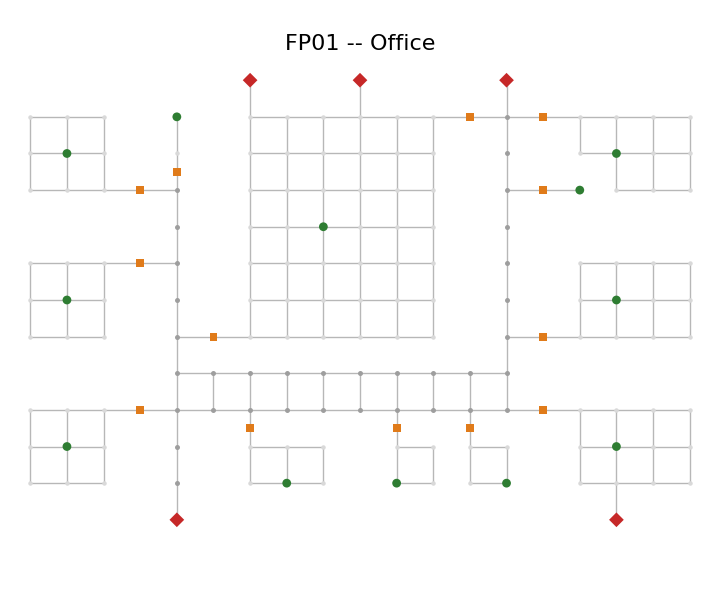
\includegraphics[width=\textwidth]{figures/blueprint_FP01.png}
\end{subfigure}
\begin{subfigure}[b]{0.32\textwidth}
\centering
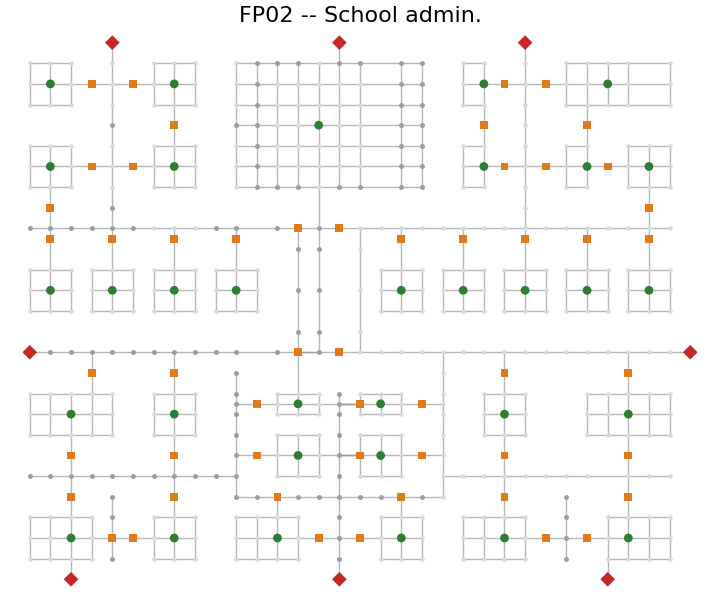
\includegraphics[width=\textwidth]{figures/blueprint_FP02.png}
\end{subfigure}
\begin{subfigure}[b]{0.32\textwidth}
\centering
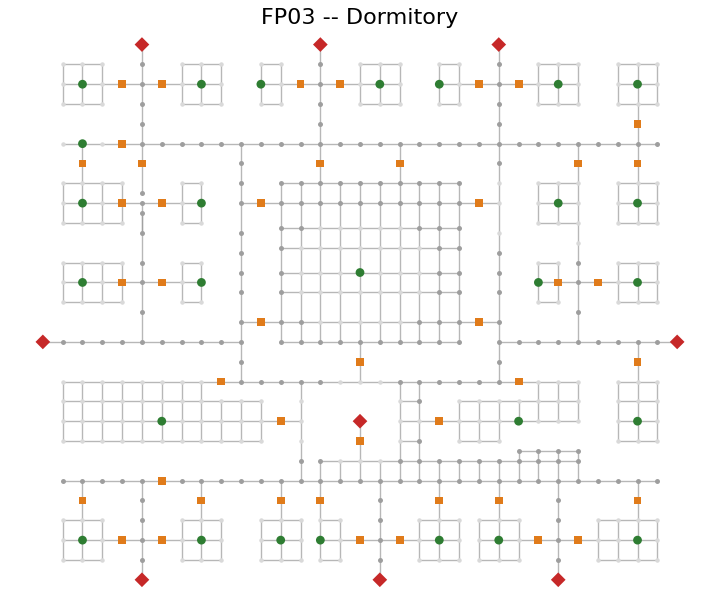
\includegraphics[width=\textwidth]{figures/blueprint_FP03.png}
\end{subfigure}

\vspace{4pt}
\begin{subfigure}[b]{0.32\textwidth}
\centering
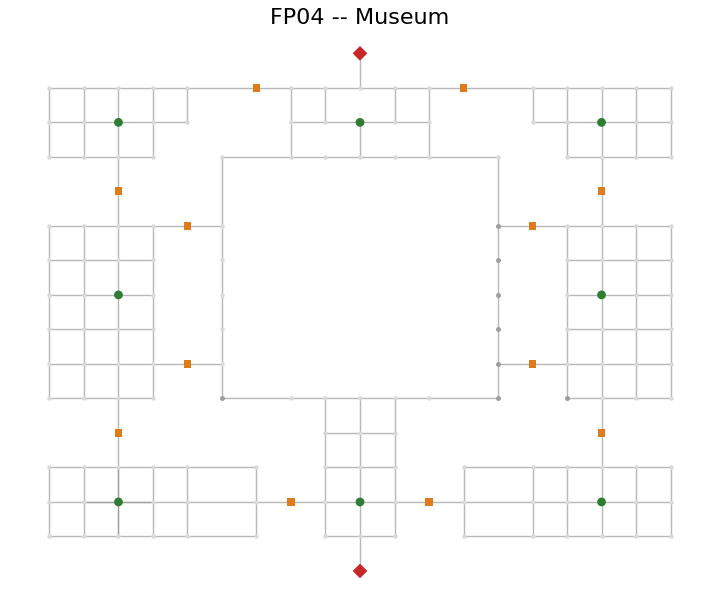
\includegraphics[width=\textwidth]{figures/blueprint_FP04.png}
\end{subfigure}
\begin{subfigure}[b]{0.32\textwidth}
\centering
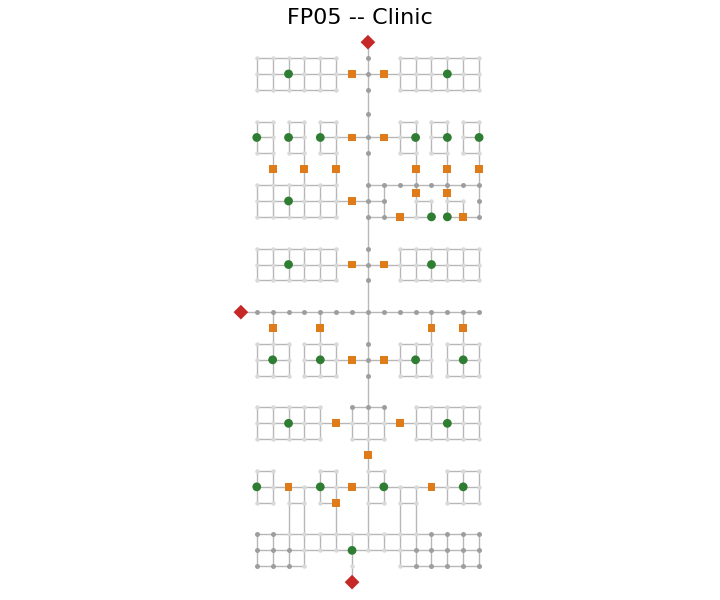
\includegraphics[width=\textwidth]{figures/blueprint_FP05.png}
\end{subfigure}
\caption{The five real floorplans (Table~\ref{tab:floorplans}). FP03's long single corridor spine and FP02's dense multi-wing layout are visually apparent here, consistent with their large certified optimality gaps (Section~\ref{sec:gaps}).}
\label{fig:blueprints-real}
\end{figure}

\begin{figure}[h]
\centering
\begin{subfigure}[b]{0.32\textwidth}
\centering
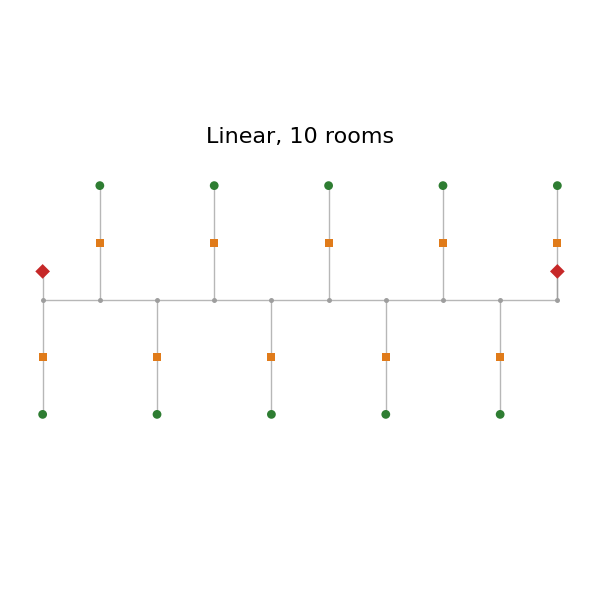
\includegraphics[width=\textwidth]{figures/blueprint_SYN_linear_10.png}
\end{subfigure}
\begin{subfigure}[b]{0.32\textwidth}
\centering
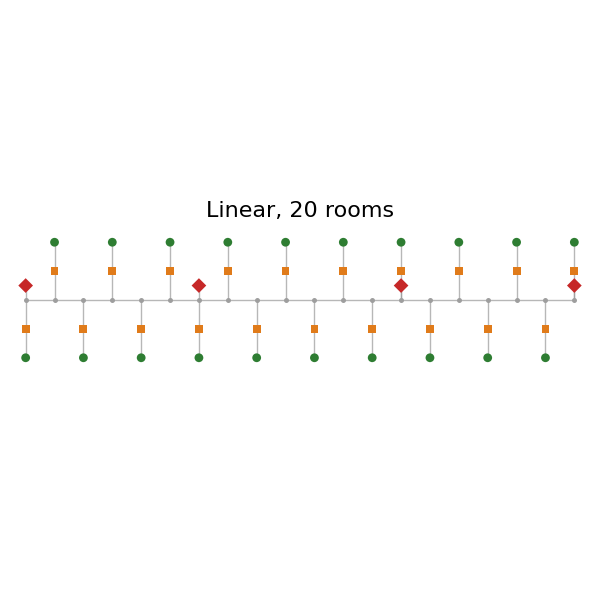
\includegraphics[width=\textwidth]{figures/blueprint_SYN_linear_20.png}
\end{subfigure}
\begin{subfigure}[b]{0.32\textwidth}
\centering
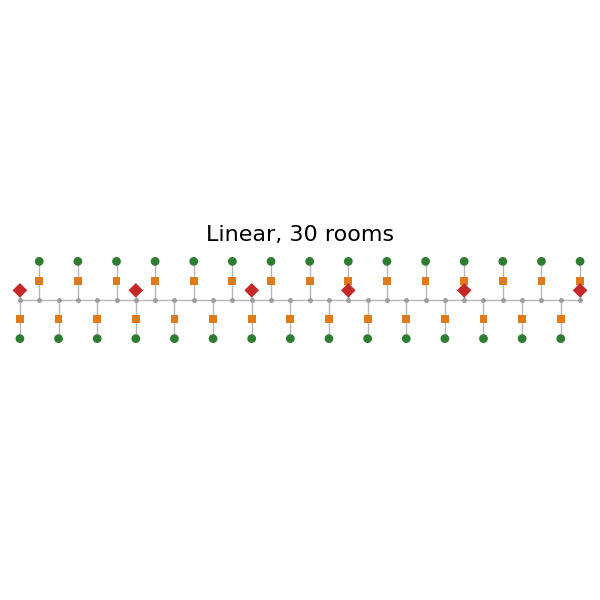
\includegraphics[width=\textwidth]{figures/blueprint_SYN_linear_30.png}
\end{subfigure}

\vspace{4pt}
\begin{subfigure}[b]{0.32\textwidth}
\centering
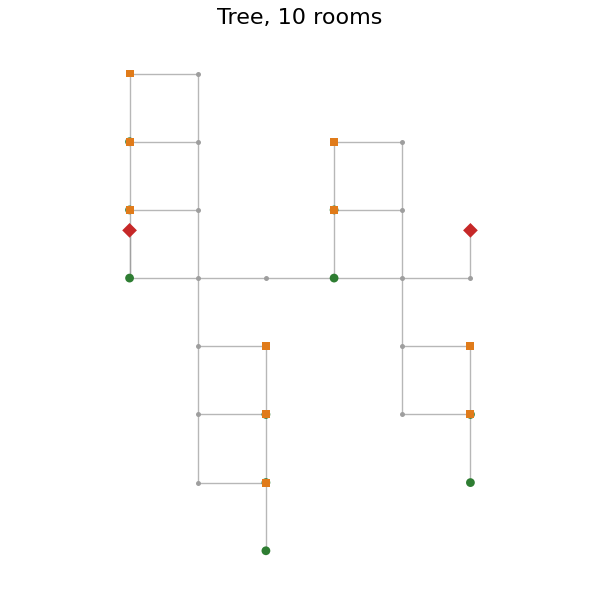
\includegraphics[width=\textwidth]{figures/blueprint_SYN_tree_10.png}
\end{subfigure}
\begin{subfigure}[b]{0.32\textwidth}
\centering
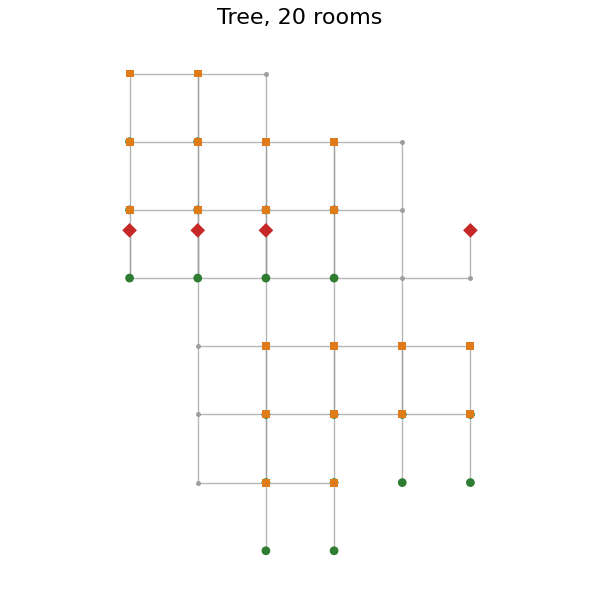
\includegraphics[width=\textwidth]{figures/blueprint_SYN_tree_20.png}
\end{subfigure}
\begin{subfigure}[b]{0.32\textwidth}
\centering
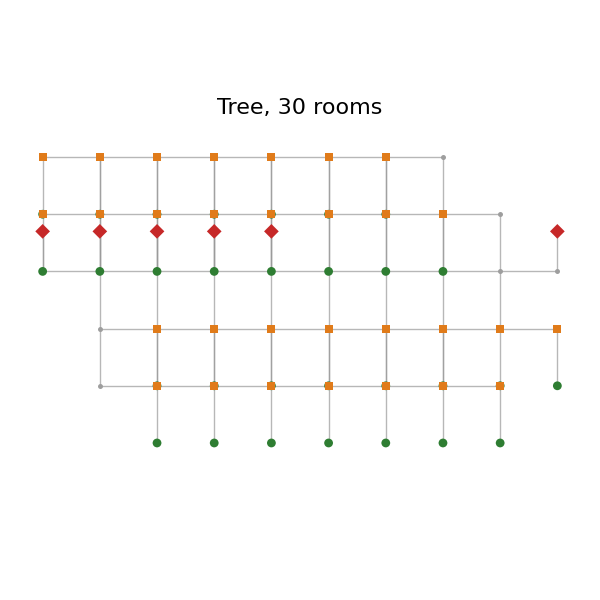
\includegraphics[width=\textwidth]{figures/blueprint_SYN_tree_30.png}
\end{subfigure}

\vspace{4pt}
\begin{subfigure}[b]{0.32\textwidth}
\centering
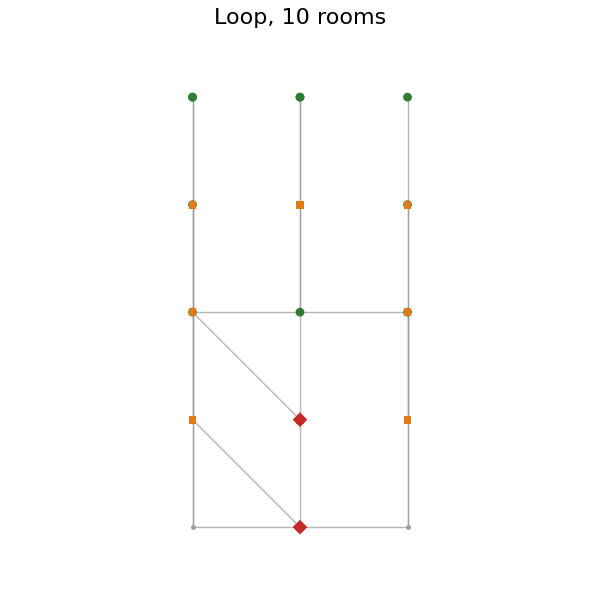
\includegraphics[width=\textwidth]{figures/blueprint_SYN_loop_10.png}
\end{subfigure}
\begin{subfigure}[b]{0.32\textwidth}
\centering
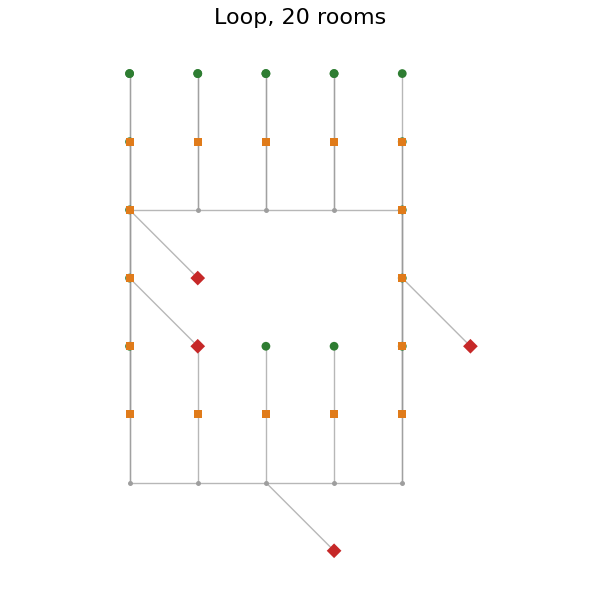
\includegraphics[width=\textwidth]{figures/blueprint_SYN_loop_20.png}
\end{subfigure}
\begin{subfigure}[b]{0.32\textwidth}
\centering
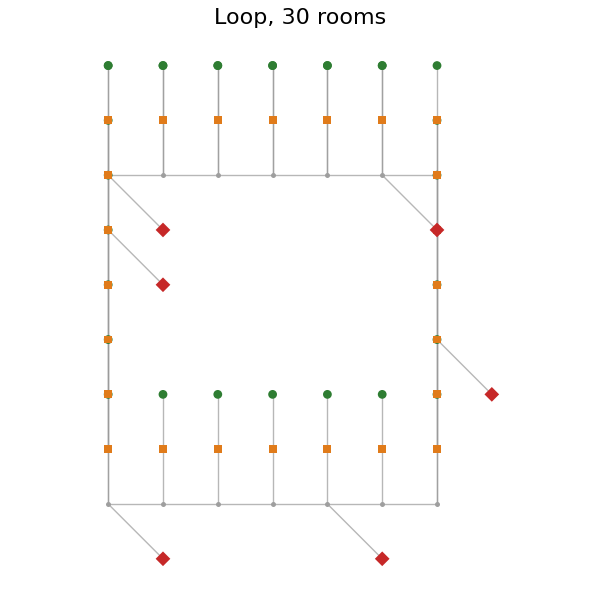
\includegraphics[width=\textwidth]{figures/blueprint_SYN_loop_30.png}
\end{subfigure}
\caption{The 9 unique synthetic layouts (rows: Linear, Tree, Loop; columns: 10, 20, 30 rooms), representative of both seeds each. Compare against Table~\ref{tab:appendixb}'s structural metrics: Linear's single spine, Tree's dual-row branch structure, and Loop's ring are all visible directly.}
\label{fig:blueprints-synthetic}
\end{figure}

\section{Reproducibility}
Source code, all 23 floorplan datasets (five real, 18 synthetic), generated route catalogs, validation tests, MILP/Neal/Hybrid benchmark outputs, blueprint figures, and this manuscript's source are available at
\begin{center}
\url{https://github.com/RomeroNatalia/EvacCapstone}, branch \path{expansion/milp-optimality-gaps},
\end{center}
forked from and building on the original study's repository at \url{https://github.com/afishman2023/EvacCapstone}.

\end{document}
